% =====================================================================
%  LectureAssist — A0 Poster  (LEFT SIDEBAR layout, left -> right)
%  Class: tikzposter (A0, portrait)  •  Compile on Overleaf with pdfLaTeX
%  ---------------------------------------------------------------------
%   • Colored LEFT title column (logo, title, authors, intro, stats,
%     pipeline). Content flows LEFT -> RIGHT in 2 columns. No top banner.
%   • Put your logo as  uni.png  next to this file.
%   • Fill in  [FILL IN: Department & University].
% =====================================================================
\documentclass[25pt, a0paper, portrait]{tikzposter}

\usepackage[utf8]{inputenc}
\usepackage[T1]{fontenc}
\usepackage{lmodern}
\usepackage{graphicx}
\usepackage{amsmath, amssymb}
\usepackage{tikz}
\usepackage{enumitem}
\usepackage{booktabs}
\usepackage{array}
\usepackage{colortbl}
\usepackage{fontawesome5}     % icons; safe to remove (fallbacks below)
\usetikzlibrary{arrows.meta, positioning, shapes.geometric, calc, fit, backgrounds}

\providecommand{\faCheckCircle}{\ensuremath{\checkmark}}
\providecommand{\faFlask}{$\bullet$}

% --------------------------------------------------------------------
%  COLOUR THEME (lighter palette)
% --------------------------------------------------------------------
\definecolor{LFindigo}{HTML}{818CF8}
\definecolor{LFindigoD}{HTML}{6366F1}
\definecolor{LFviolet}{HTML}{A78BFA}
\definecolor{LFcyan}{HTML}{38BDF8}
\definecolor{LFgreen}{HTML}{34D399}
\definecolor{LFamber}{HTML}{FBBF24}
\definecolor{LFred}{HTML}{F87171}
\definecolor{LFink}{HTML}{2B2C45}
\definecolor{LFmist}{HTML}{F4F5FD}
\definecolor{LFmist2}{HTML}{EAEDFC}
\definecolor{LFpaper}{HTML}{FCFCFE}

\definecolorstyle{LectureAssist}{}{
  \colorlet{backgroundcolor}{LFpaper}
  \colorlet{framecolor}{LFindigo}
  \colorlet{titlefgcolor}{white}
  \colorlet{titlebgcolor}{LFindigo}
  \colorlet{blocktitlebgcolor}{LFindigo}
  \colorlet{blocktitlefgcolor}{white}
  \colorlet{blockbodybgcolor}{white}
  \colorlet{blockbodyfgcolor}{LFink}
  \colorlet{innerblocktitlebgcolor}{LFmist2}
  \colorlet{innerblocktitlefgcolor}{LFindigoD}
  \colorlet{innerblockbodybgcolor}{LFmist}
  \colorlet{innerblockbodyfgcolor}{LFink}
  \colorlet{notebgcolor}{LFviolet}
  \colorlet{notefgcolor}{white}
  \colorlet{notefrcolor}{LFviolet}
}
\usecolorstyle{LectureAssist}

\usetitlestyle{Empty}
\useblockstyle{Default}

% subtle light gradient background
\definebackgroundstyle{LFbg}{
  \draw[inner sep=0, line width=0, top color=LFmist, bottom color=LFpaper]
    (bottomleft) rectangle (topright);
}
\usebackgroundstyle{LFbg}

% --------------------------------------------------------------------
%  TIKZ NODE STYLES
% --------------------------------------------------------------------
\tikzset{
  lfbox/.style={
    rectangle, rounded corners=10pt, draw=LFindigoD, line width=1.4pt,
    fill=white, text=LFink, align=center, inner sep=10pt, minimum height=1.9cm,
    font=\large\bfseries},
  lfin/.style={lfbox, draw=LFcyan, fill=LFmist},
  lfproc/.style={lfbox, draw=LFviolet},
  lfllm/.style={lfbox, draw=LFamber, fill=LFamber!10},
  lfout/.style={lfbox, draw=LFgreen, fill=LFgreen!8},
  lfarr/.style={-{Stealth[length=6mm,width=5mm]}, line width=1.6pt, draw=LFindigoD},
  lfarrg/.style={-{Stealth[length=6mm,width=5mm]}, line width=1.6pt, draw=LFgreen},
  lfloop/.style={-{Stealth[length=5mm,width=4mm]}, line width=1.4pt, draw=LFviolet},
  lflbl/.style={font=\normalsize\itshape, text=LFink!70, fill=white, inner sep=2pt},
  sbox/.style={rectangle, rounded corners=8pt, fill=white, text=LFindigoD,
    align=center, inner sep=8pt, minimum height=1.5cm, font=\large\bfseries,
    text width=6.0cm},
  sarr/.style={-{Stealth[length=6mm,width=5mm]}, line width=1.8pt, draw=white},
}

\newcommand{\secnum}[1]{\tikz[baseline=-0.55ex]\node[circle, fill=LFviolet,
  text=white, font=\bfseries\large, minimum size=1.05cm, inner sep=0]{#1};}

\newcommand{\stat}[2]{%
  \begin{minipage}[t]{0.48\linewidth}\centering
  {\fontsize{30}{32}\selectfont\bfseries #1}\\[1pt]
  {\small #2}\end{minipage}}

\title{}
\author{}
\settitle{}

\begin{document}

\maketitle[titletotopverticalspace=0mm, titletoblockverticalspace=0mm,
           titlegraphictotitledistance=0mm]

% ====================================================================
%  COLUMNS  (title lives in the left sidebar)
% ====================================================================
\begin{columns}

% ============ COLUMN 1 : COLORED TITLE SIDEBAR ======================
\column{0.30}
{% local recolor: light indigo band with dark text
\colorlet{blocktitlebgcolor}{LFindigoD}
\colorlet{blockbodybgcolor}{LFmist2}
\colorlet{blockbodyfgcolor}{LFink}
\block{\color{white}LectureAssist}{%
\begin{minipage}[t]{\linewidth}
\centering
\IfFileExists{uni.png}
  {
\includegraphics[width=0.75\linewidth, height=4.5cm, keepaspectratio]{uni.png}}
  {\fcolorbox{LFindigoD}{white}{\parbox[c][2.4cm][c]{0.58\linewidth}{\centering
     \color{LFindigoD}\bfseries UNIVERSITY LOGO\\[2pt]{\footnotesize add uni.png}}}}
\\[8pt]
{\large\bfseries\color{LFindigoD} An Agentic, Multimodal AI Assistant\\ that Turns Lectures into Adaptive Study Material}
\\[7pt]
{\normalsize Iftikhar Ahmed \;\textbullet\; Salman Shafi \;\textbullet\; Jarinah Tasnim}\\[3pt]
{\small\itshape Dept.\ of Electrical and Computer Engineering\\North South University}\\[2pt]
{\small Senior Design Project (499)}
\par\vspace{9pt}
{\color{LFindigoD}\hrule height 1.5pt}\vspace{8pt}

\raggedright
\textbf{\normalsize Overview.}\; LectureAssist turns a lecture \textbf{video} or
\textbf{document} into a summary, multi-format quizzes, flashcards, exam hints
and a grounded chat tutor. Cooperating \textbf{LLM agents} plan, generate,
\emph{validate} and refine every artifact; a \textbf{RAG} index keeps answers
anchored to the real lecture. Everything runs on one \textbf{free Colab T4 GPU}
with a \textbf{local} Gemma-3 model --- no paid API.
\par\vspace{9pt}
{\color{LFindigoD}\hrule height 1.5pt}\vspace{8pt}

\centering
\stat{\$0}{API cost (local LLM)}\hfill\stat{100\%}{RAG-grounded + cited}\\[8pt]
\stat{5}{quiz / study types}\hfill\stat{EN·BN}{OCR languages}
\par\vspace{8pt}
{\color{LFindigoD}\hrule height 1.5pt}\vspace{8pt}

\textbf{\normalsize End-to-End Pipeline}\\[6pt]
\resizebox{0.88\linewidth}{!}{%
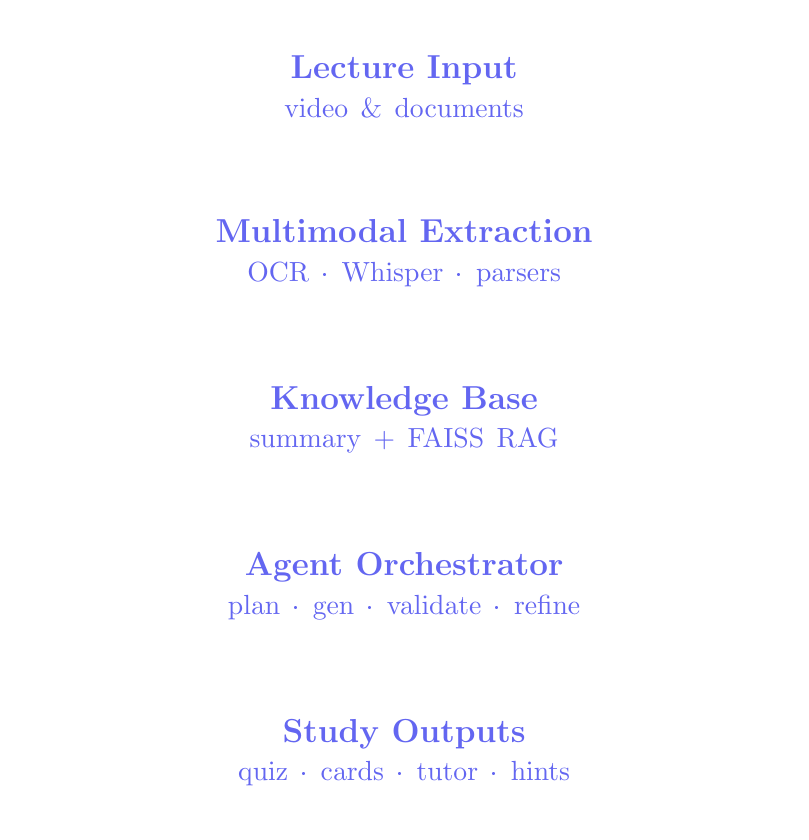
\begin{tikzpicture}[node distance=0.6cm]
  \node[sbox, text width=9.0cm] (in){Lecture Input\\{\normalfont\normalsize video \& documents}};
  \node[sbox, text width=9.0cm, below=of in] (ex){Multimodal Extraction\\{\normalfont\normalsize OCR · Whisper · parsers}};
  \node[sbox, text width=9.0cm, below=of ex] (kb){Knowledge Base\\{\normalfont\normalsize summary + FAISS RAG}};
  \node[sbox, text width=9.0cm, below=of kb] (ag){Agent Orchestrator\\{\normalfont\normalsize plan · gen · validate · refine}};
  \node[sbox, text width=9.0cm, below=of ag] (ou){Study Outputs\\{\normalfont\normalsize quiz · cards · tutor · hints}};
  \draw[sarr](in)--(ex); \draw[sarr](ex)--(kb);
  \draw[sarr](kb)--(ag); \draw[sarr](ag)--(ou);
\end{tikzpicture}}
\par\vspace{6pt}
{\small Flask on Colab $\to$ ngrok $\to$ browser UI.}
\par\vspace{10pt}
{\color{LFindigoD}\hrule height 1.5pt}\vspace{8pt}

\raggedright
\textbf{\large Technology Stack}\\[6pt]
{\normalsize
\textbf{Reasoning:} Ollama · Gemma\,3 (12B/4B).\\[3pt]
\textbf{Vision/Audio:} EasyOCR · OpenCV · Faster-Whisper.\\[3pt]
\textbf{Retrieval:} Sentence-Transformers · FAISS.\\[3pt]
\textbf{Docs:} PyMuPDF · docx · pptx.\\[3pt]
\textbf{Serving:} Flask · CORS · pyngrok (Colab T4).\\[3pt]
\textbf{Storage:} Google Drive.}
\end{minipage}
}%
}% end recolor group

% ============ COLUMN 2 ==============================================
\column{0.35}

\block{\secnum{1}\; Motivation \& Problem}{
Students re-watch hours of recorded lectures to find one concept, and have no
fast way to self-test on the material a teacher emphasised.
\begin{itemize}[leftmargin=*, itemsep=3pt]
  \item Lecture knowledge is locked in \textbf{video, speech and slides} --- rarely clean text.
  \item Generic quiz tools \textbf{hallucinate} off-topic questions.
  \item One-size difficulty ignores \textbf{each student's weak spots}.
\end{itemize}
\textbf{Goal:} an offline-capable system that \emph{reads the board, hears the
lecture}, and produces \emph{grounded, validated, adaptive} study tools.
}

\block{\secnum{2}\; Multimodal Extraction}{
Every modality is recovered and time-aligned before any LLM call.
\begin{itemize}[leftmargin=*, itemsep=3pt]
  \item \textbf{Visual / OCR (EasyOCR).} Frames sampled $\sim$5\,s apart, then
        \emph{classified} (slide / blackboard / whiteboard / scene) with per-class
        preprocessing (CLAHE, sharpening, Otsu, chalk inversion). \textbf{EN + BN}.
  \item \textbf{Speech (Faster-Whisper).} GPU \texttt{float16} / CPU \texttt{int8}
        fallback, VAD filtering, per-segment timestamps.
  \item \textbf{Documents.} PyMuPDF, python-docx, python-pptx (structure kept).
  \item \textbf{Drive OCR cache} by video hash --- re-uploads skip re-scan.
\end{itemize}
}

\block{\secnum{3}\; Multi-Agent Orchestration}{
A central \textbf{Orchestrator} runs specialist agents; independent ones run
\textbf{concurrently}. Each follows: \texttt{should\_run $\to$ plan $\to$ execute
$\to$ validate $\to$ retry}.
\vspace{3.0cm}
\begin{center}
\resizebox{0.55\linewidth}{!}{%
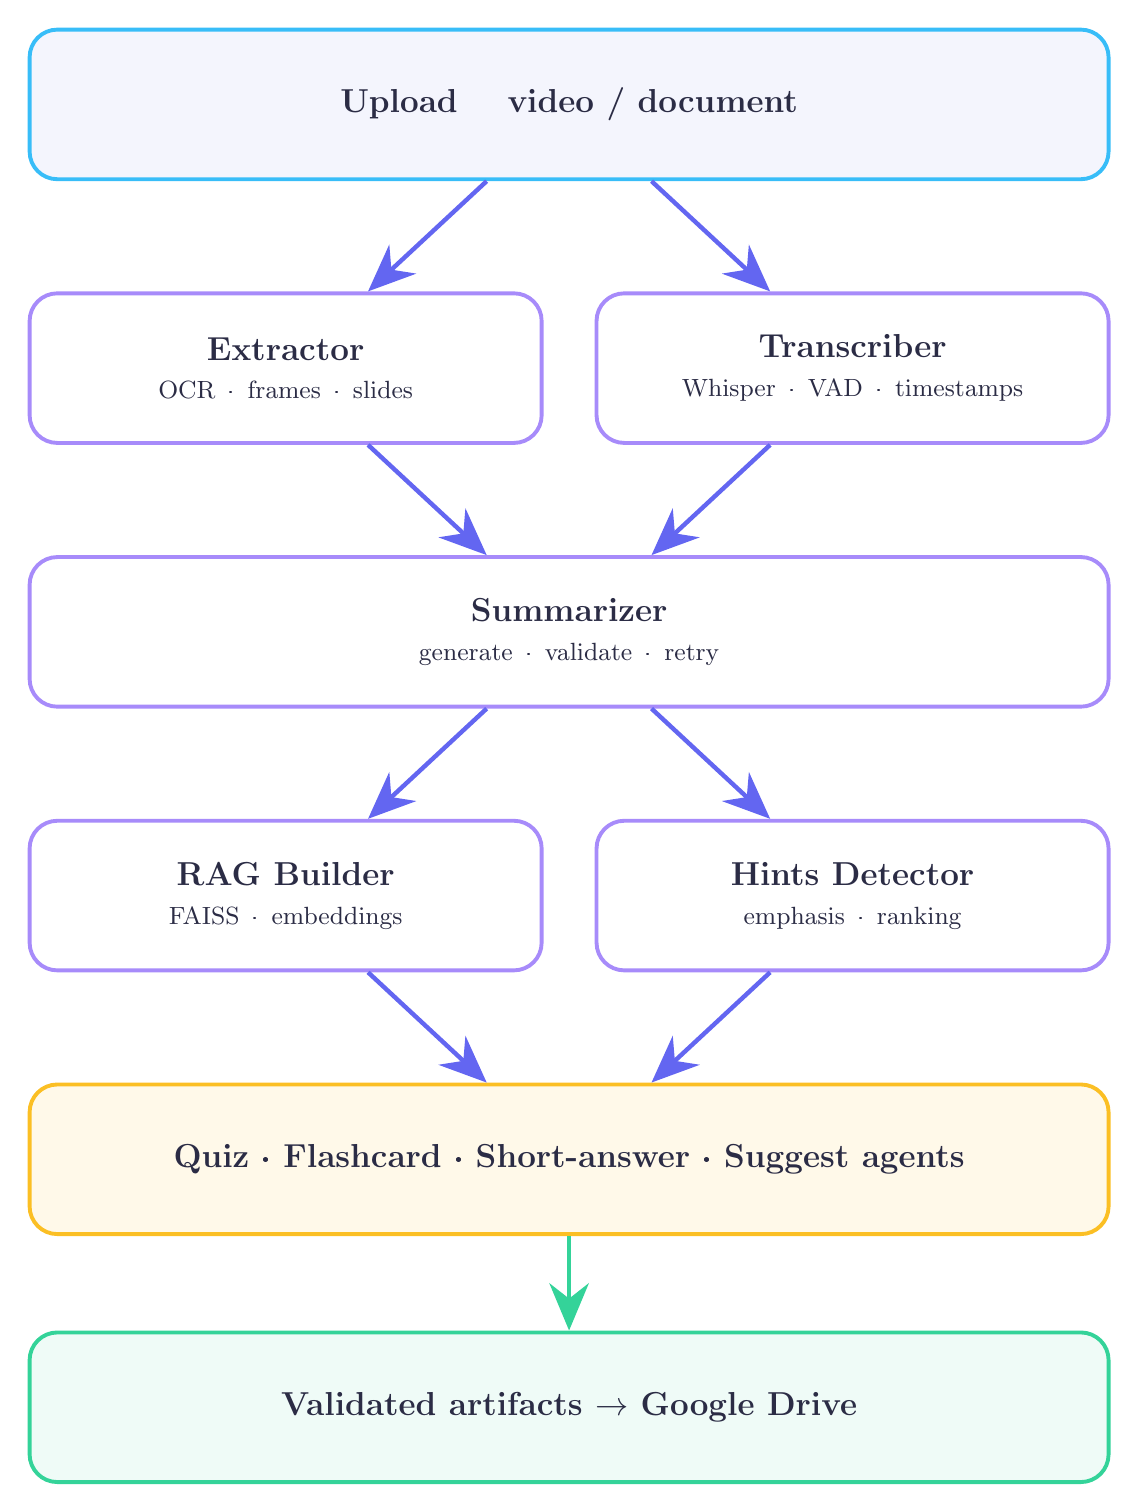
\begin{tikzpicture}[font=\large]
  %% Row 1: Upload
  \node[lfin, text width=13cm] (s0)
        {\textbf{Upload} \quad video / document};
  %% Row 2: Extractor + Transcriber
  \node[lfproc, text width=5.8cm, below=1.4cm of s0, xshift=-3.6cm] (a)
        {Extractor\\{\normalfont\small OCR · frames · slides}};
  \node[lfproc, text width=5.8cm, below=1.4cm of s0, xshift= 3.6cm] (b)
        {Transcriber\\{\normalfont\small Whisper · VAD · timestamps}};
  %% Row 3: Summarizer (re-centred using a + xshift)
  \node[lfproc, text width=13cm, below=1.4cm of a, xshift=3.6cm] (sum)
        {Summarizer\\{\normalfont\small generate · validate · retry}};
  %% Row 4: RAG Builder + Hints Detector
  \node[lfproc, text width=5.8cm, below=1.4cm of sum, xshift=-3.6cm] (rag)
        {RAG Builder\\{\normalfont\small FAISS · embeddings}};
  \node[lfproc, text width=5.8cm, below=1.4cm of sum, xshift= 3.6cm] (hint)
        {Hints Detector\\{\normalfont\small emphasis · ranking}};
  %% Row 5: Quiz agents
  \node[lfllm, text width=13cm, below=1.4cm of rag, xshift=3.6cm] (quiz)
        {\textbf{Quiz} · Flashcard · Short-answer · Suggest agents};
  %% Row 6: Output
  \node[lfout, text width=13cm, below=1.2cm of quiz] (done)
        {Validated artifacts $\to$ Google Drive};
  %% Arrows
  \draw[lfarr](s0)--(a);  \draw[lfarr](s0)--(b);
  \draw[lfarr](a)--(sum); \draw[lfarr](b)--(sum);
  \draw[lfarr](sum)--(rag); \draw[lfarr](sum)--(hint);
  \draw[lfarr](rag)--(quiz); \draw[lfarr](hint)--(quiz);
  \draw[lfarrg](quiz)--(done);
\end{tikzpicture}}
\end{center}
\vspace{4pt}
{\small Any agent crash is caught \& logged --- the pipeline degrades gracefully.}
}

% ============ COLUMN 3 ==============================================
\column{0.34}

\block{\secnum{5}\; Grounded Retrieval (RAG)}{
\begin{minipage}[c]{0.46\linewidth}
\raggedright
Speech \& board/slide text are embedded with \textbf{Sentence\-Transformers}
(\texttt{MiniLM}) and indexed in \textbf{FAISS} (cosine). Every quiz, summary and
chat answer retrieves \textbf{top-$k$} chunks first --- \emph{anchored} to real
content with a clickable \textbf{timestamp}.
\end{minipage}\hfill
\begin{minipage}[c]{0.50\linewidth}\centering
\resizebox{0.90\linewidth}{!}{%
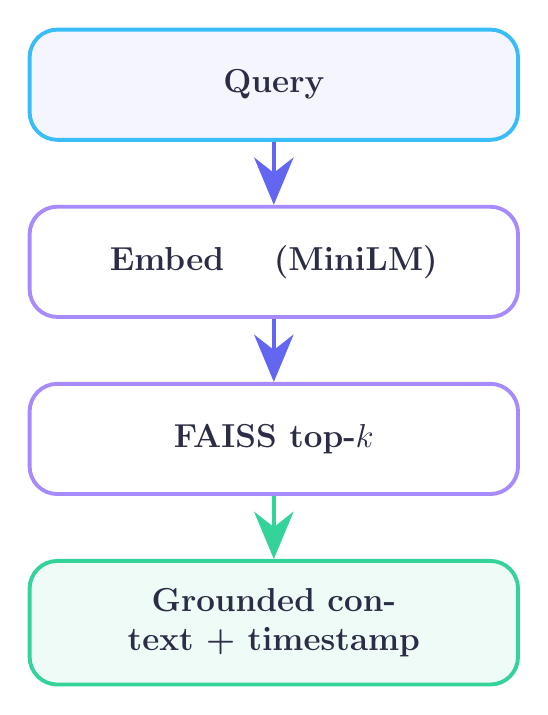
\begin{tikzpicture}[node distance=0.8cm, font=\large]
  \node[lfin,   text width=5.5cm, minimum height=1.4cm] (q){Query};
  \node[lfproc, below=of q,   text width=5.5cm, minimum height=1.4cm] (emb){Embed \quad (MiniLM)};
  \node[lfproc, below=of emb, text width=5.5cm, minimum height=1.4cm] (fa){FAISS top-$k$};
  \node[lfout,  below=of fa,  text width=5.5cm, minimum height=1.5cm] (c){Grounded context + timestamp};
  \draw[lfarr](q)--(emb);\draw[lfarr](emb)--(fa);\draw[lfarrg](fa)--(c);
\end{tikzpicture}}
\end{minipage}
}

\block{\secnum{6}\; Adaptive \& Socratic Learning}{
\begin{itemize}[leftmargin=*, itemsep=3pt]
  \item \textbf{Self-improving difficulty.} A \emph{Difficulty Adapter} tracks
        per-topic accuracy, flags weak topics ($<$50\%), steers the planner there.
  \item \textbf{Socratic tutor.} Asks guiding questions; reveals the full answer
        only after \textbf{2 attempts} or ``just tell me''. Cites timestamps,
        plays the exact \textbf{video clip} inline.
  \item \textbf{AI short-answer grading} with partial credit \& feedback.
\end{itemize}
}

\block{\secnum{7}\; Key Features}{
\begin{itemize}[leftmargin=*, itemsep=2pt]
  \item 5 artifacts: \textbf{MCQ, T/F, Fill-blank, Short-answer, Flashcards}.
  \item \textbf{Exam-hint detection} from teacher emphasis cues + topic ranking.
  \item \textbf{Timestamped video clips} on demand (ffmpeg + HTTP range).
  \item \textbf{Lecture timeline} merging speech \& board text.
  \item \textbf{Session persistence \& auto-restore} (Drive).
  \item \textbf{Lesson planner} + \textbf{print/PDF export}.
\end{itemize}
}

\block{\secnum{8}\; Results \& Capabilities}{
{\small\renewcommand{\arraystretch}{1.15}
\begin{tabular}{>{\raggedright\arraybackslash}p{0.52\linewidth} >{\raggedright\arraybackslash}p{0.40\linewidth}}
\toprule
\rowcolor{LFmist2}\textbf{Capability} & \textbf{Outcome}\\
\midrule
Input formats & 5 video + 3 doc\\
OCR languages & EN + BN\\
Per-question checks & 4, $\le 3$ retries\\
Quiz / study types & 5\\
Grounding & 100\% + timestamp\\
LLM hosting & local, \$0 API\\
Cached OCR re-runs & skipped\\
Agent failures & isolated\\
\bottomrule
\end{tabular}}
\\[4pt]
\colorbox{LFmist}{\parbox{0.95\linewidth}{\small \faFlask\;
\textbf{Eval (to complete):} add measured numbers --- acceptance rate,
validator vs.\ human, OCR/WER, T4 runtime.}}
}

\end{columns}

% ====================================================================
%  FULL-WIDTH ROW: Agentic Quiz Generation
% ====================================================================
\block{\secnum{4}\; Agentic Quiz Generation}{
\begin{minipage}[c]{0.32\linewidth}
\raggedright
Questions are built \textbf{one at a time} and must \emph{pass validation} before
the next --- eliminating hallucinated, off-topic or duplicate questions.
\vspace{10pt}

\textbf{Validation gate:}\\[4pt]
\faCheckCircle\; grounded in lecture\\[3pt]
\faCheckCircle\; right difficulty\\[3pt]
\faCheckCircle\; follows instructions\\[3pt]
\faCheckCircle\; not duplicate ($>$85\%)
\vspace{10pt}

\textbf{Modes:} \emph{Auto} $\cdot$ \emph{Manual}
(Easy / Med / Hard) $\cdot$ \emph{Adaptive}
(targets weak topics).\\[4pt]
Live ``thinking'' streamed to the UI.
\end{minipage}%
\hfill
\begin{minipage}[c]{0.64\linewidth}
\centering
\resizebox{0.62\linewidth}{!}{%
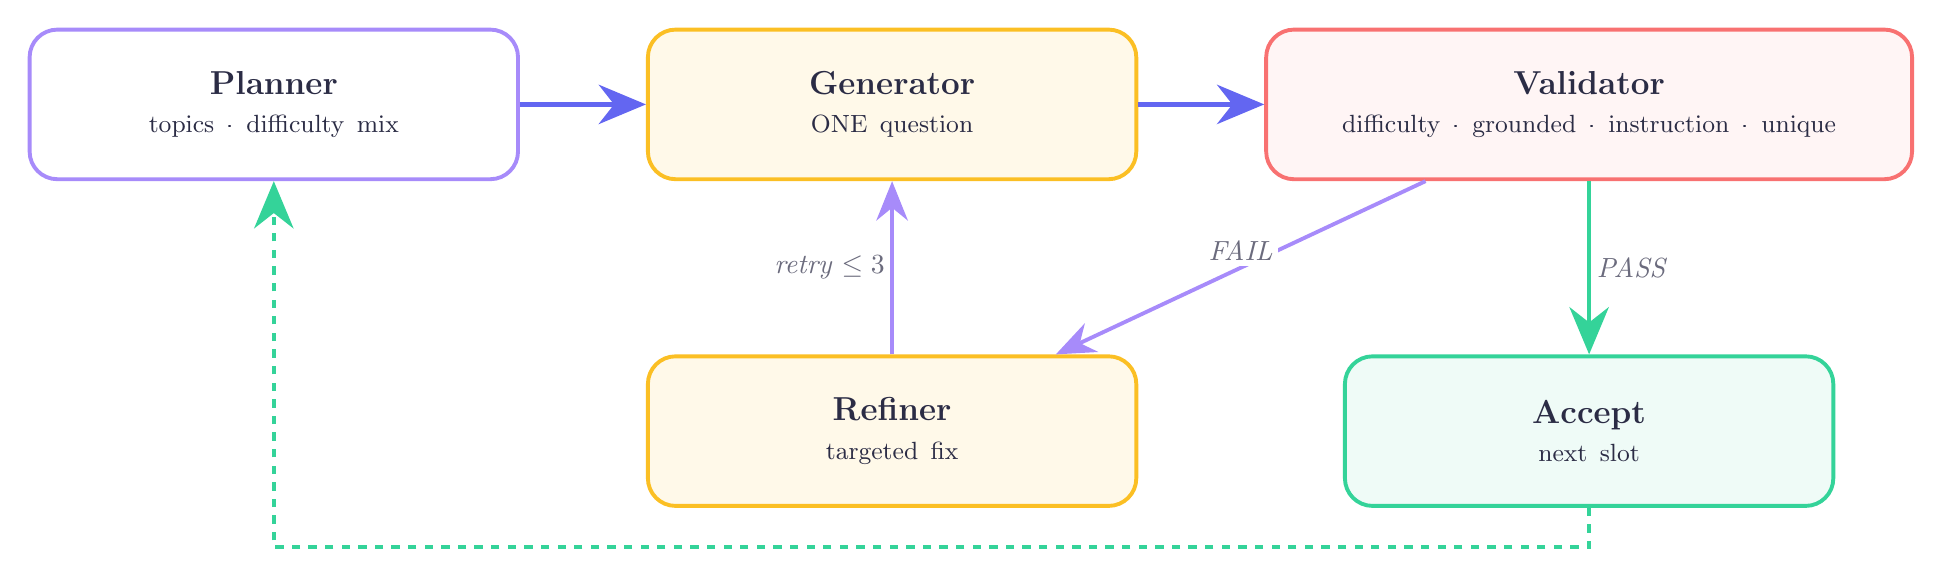
\begin{tikzpicture}[node distance=1.1cm, font=\normalsize]
  %% Top row
  \node[lfproc, text width=5.5cm] (plan)
        {\textbf{Planner}\\{\normalfont\small topics · difficulty mix}};
  \node[lfllm, right=1.6cm of plan, text width=5.5cm] (gen)
        {\textbf{Generator}\\{\normalfont\small ONE question}};
  \node[lfbox, draw=LFred, fill=LFred!7, right=1.6cm of gen, text width=7.5cm] (val)
        {\textbf{Validator}\\{\normalfont\small difficulty · grounded · instruction · unique}};
  %% Bottom row
  \node[lfbox, draw=LFamber, fill=LFamber!10, below=2.2cm of gen, text width=5.5cm] (refine)
        {\textbf{Refiner}\\{\normalfont\small targeted fix}};
  \node[lfout, below=2.2cm of val, text width=5.5cm] (pass)
        {\textbf{Accept}\\{\normalfont\small next slot}};
  %% Arrows
  \draw[lfarr](plan)--(gen);
  \draw[lfarr](gen)--(val);
  \draw[lfarrg](val)--(pass)  node[lflbl, midway, right]{PASS};
  \draw[lfloop](val)--(refine) node[lflbl, midway, above]{FAIL};
  \draw[lfloop](refine)--(gen) node[lflbl, midway, left]{retry $\le 3$};
  \draw[lfarrg, dashed](pass.south) -- ++(0,-0.5) -| (plan.south);
\end{tikzpicture}}
\end{minipage}
}

\end{document}
